\section{Analytical results}

\subsection{Transfer orbit}

\begin{figure}[h]
    \centering
    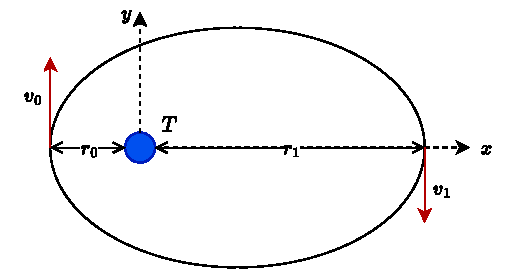
\includegraphics[width=0.6\linewidth]{figures/transfert.pdf}
    \caption{Schematic of the transfer orbit of Webb}
    \label{fig:schema_transfert}
\end{figure}
In this first part we only consider the gravitational pull from the Earth. We would like to calculate the speed needed for Webb to reach a distance \(r_1 = 1.5\) million km at the peak of the transfer orbit, starting from a lower distance \(r_0 = 6800\) km as shown in \autoref{fig:schema_transfert}. Let \(m\) be the mass of Webb, \(m_T\) the mass of the Earth, \(v_0\) and \(v_1\) the required start and end speed respectively. From conservation of TODO, we can write
\begin{equation}
    r_0 v_0 = r_1 v_1
    \label{eq:conservation_moment_inertie}
\end{equation}
and using conservation of energy
\begin{equation}
    \frac{1}{2} m v_0^2 - G \frac{m m_T}{r_0} = \frac{1}{2} m v_1^2 - G \frac{m m_T}{r_1}
    \label{eq:conservation_energy}
\end{equation}
where \(G = 6.674 \cdot 10{-11}\) \si{\meter\cubed\per\kilo\gram\per\second\squared}. Using \autoref{eq:conservation_moment_inertie} we get
\begin{equation}
    v_0 = \frac{r_1 v_1}{r_0}
    \label{eq:v0_substitution}
\end{equation}
which we can then substitute in \autoref{eq:conservation_energy} to get
\begin{equation}
    \frac{1}{2} m \left(\frac{r_1}{r_0}\right)^2 v_1^2 - G \frac{m m_T}{r_0} = \frac{1}{2} m v_1^2 - G \frac{m m_T}{r_1}
\end{equation}
Solving for \(v_1\) we get the following expression:
\begin{equation}
    v_1 = r_0 \sqrt{2 G m_T \frac{\frac{1}{r_0}-\frac{1}{r_1}}{r_1^2-r_0^2}}
\end{equation}
Using \autoref{eq:v0_substitution}, we have
\begin{equation}
    v_0 = r_1 \sqrt{2 G m_T \frac{\frac{1}{r_0}-\frac{1}{r_1}}{r_1^2-r_0^2}}
\end{equation}
Evaluating these expressions using \(m_T = 5.9736 \cdot 10^{24}\) kg gives us
\begin{equation}
    v_0 \approx 10804 \, \textrm{m/s} \quad v_1 \approx 49 \, \textrm{m/s}
\end{equation}

We now want to obtain the equations of motion of Webb. Let us take the vector \(\mathbf{y} = (x(t), y(t), \dot x(t), \dot y(t))\). We are searching for \(\mathbf{f}\) such that:
\begin{equation}
    \frac{\dd \mathbf{y}}{\dd t} = \left(\begin{matrix} \dot x \\ \dot y \\ \ddot x \\ \ddot y \end{matrix}\right) = \mathbf{f}(\mathbf{y})
\end{equation}
The only force applied on Webb is the gravitational pull of the Earth. The equations of motion along \(x\) and \(y\) are:
\begin{equation}
    \begin{cases}
        m \ddot x = -G \frac{m m_T}{\left(x^2+y^2\right)^\frac{3}{2}} x \\
        m \ddot y = -G \frac{m m_T}{\left(x^2+y^2\right)^\frac{3}{2}} y
    \end{cases}
\end{equation}
Which allows us to express \(\mathbf{f}(\mathbf{y})\) as
\begin{equation}
    \frac{\dd \mathbf{y}}{\dd t} = \mathbf{f}(\mathbf{y}) = \left(\begin{matrix} \dot x \\ \dot y \\ -G \frac{m_T}{\left(x^2+y^2\right)^\frac{3}{2}} x \\ -G \frac{m_T}{\left(x^2+y^2\right)^\frac{3}{2}} y \end{matrix}\right).
\end{equation}

\subsection{Sun-Earth system}

Consider the Sun-Earth system, where \(m_S = 1.98892 \cdot 10^{30}\) kg and \(m_T = 5.9736 \cdot 10^{24}\) kg are the respective masses of these objects. Supposing a constant distance \(d = 149598023\) km between the Sun and the Earth and a circular orbit, we want to obtain the position of the Sun \(x_S'\) and Earth \(x_T'\) relative to their center of mass \(\mathcal G\). We position the axis \(x'\) as the Sun-Earth axis, where the center of mass \(\mathcal G\) is at \(x'=0\). This coordinate system is shown in \autoref{fig:schema_referentiel}.
\begin{figure}[h]
    \centering
    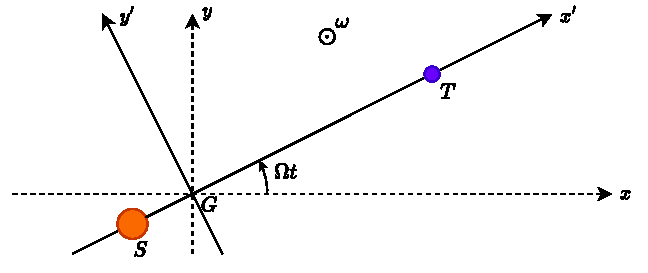
\includegraphics[width=0.8\linewidth]{figures/referentiel.pdf}
    \caption{Schematic of the transfer orbit of Webb}
    \label{fig:schema_referentiel}
\end{figure}
Using the equation for the position of the center of mass, i.e.
\begin{equation}
    \begin{aligned}
        &\mathcal G = \frac{x_T' m_T + x_S' m_S}{m_T + m_S} \stackrel{!}{=} 0 \\
        &\implies x_T' m_T + x_S' m_S = 0
    \end{aligned}
\end{equation}
and the fact that the distance between the Sun and Earth is given by \(|x_T'|+|x_S'| = x_T' - x_S' = d\), where the minus sign is because \(x_S'\) is on the left hand side of \(\mathcal G\), we get a system of equations
\begin{equation}
    \begin{cases}
        x_T' - x_S' = d \\
        x_T' m_T = -x_S' m_S
    \end{cases}
\end{equation}
Solving this system gives us the positions of the Sun and Earth in this new coordinate system
\begin{equation}
    x_T' = \frac{m_S d}{m_T + m_S}, \quad x_S' = \frac{m_T d}{m_T + m_S}
\end{equation}

We would also like to know angular speed \(\Omega\) of the planets. Using the circular orbit hypothesis, we get that the motion is circular uniform. This allows us to express the norm of the acceleration \(a\) as \(a = \frac{v^2}{r}\), where \(v^2\) is the squared norm of the speed of the planet and \(r\) is the radius of its orbit. Because \(v = \Omega r\), we have \(a = \Omega^2 r\). Furthermore, using \(\vec F=m \vec a \implies a = \left|\frac{F}{m}\right|\), we get for the orbit of the Earth
\begin{equation}
    \left|\frac{F}{m_T}\right| = G \frac{m_S}{d^2} = \Omega^2 x_T'
\end{equation}
which gives an expression for the angular speed \(\Omega\)
\begin{equation}
    \Omega = \sqrt{G \frac{m_S}{d^2 x_T'}}
\end{equation}
where only the positive root was taken because we the motion to be counter-clockwise, as shown in \autoref{fig:schema_referentiel}. We denote the rotation vector \(\vec\Omega = (0, 0, \Omega)\). Evaluating numerically, we get \(\Omega \approx 1.99 \cdot 10^{-7}\) rad/s, which does give an orbital period \(T = \frac{2 \pi}{\Omega} \approx 365.2\) days as expected.

\subsection{Equations of motion in rotating frame of reference}
\label{sec:3body_reduced}

Let \(\mathcal R'\) be a rotating frame of reference at angular speed \(\Omega\), with a cartesian coordinate system \((x',y')\) centered in \(\mathcal G\). In this frame, the Sun and Earth are motionless. We want to obtain the equations of motion of Webb in this reference frame. Let us take the vector \(\mathbf{y} = (x'(t), y'(t), \dot x'(t), \dot y'(t))\). We are searching for \(\mathbf{f}\) such that:
\begin{equation}
    \frac{\dd \mathbf{y}}{\dd t} = \left(\begin{matrix} \dot x' \\ \dot y' \\ \ddot x' \\ \ddot y' \end{matrix}\right) = \mathbf{f}(\mathbf{y})
\end{equation}
We denotate the position of Webb as \(\vec{r}\,' = (x', y', 0)\). The forces acting on the satelite are:
\begin{enumerate}
    \item The gravitational pull from the Earth:
    \begin{equation}
        -G \frac{m m_T}{|\vec{r}\,' - \vec{r_T}'|^3} (\vec{r}\,' - \vec{r_T}')
    \end{equation}
    where \(\vec{r_T}' = (x_T', 0, 0)\)
    \item The gravitational pull from the Sun:
    \begin{equation}
        -G \frac{m m_S}{|\vec{r}\,' - \vec{r_S}'|^3} (\vec{r}\,' - \vec{r_S}')
    \end{equation}
    where \(\vec{r_S}' = (x_S', 0, 0)\)
    \item The Coriolis force:
    \begin{equation}
        -2 m \vec\Omega \times \frac{\dd \vec{r}\,'}{\dd t} = 2 m \left(\begin{matrix} \Omega \dot y' \\ -\Omega \dot x' \\ 0 \end{matrix}\right)
    \end{equation}
    \item The centrifugal force:
    \begin{equation}
        -m \vec\Omega \times (\vec\Omega \times \vec{r}\,') = m \Omega^2 \left(\begin{matrix} x' \\ y' \\ 0 \end{matrix}\right)
    \end{equation}
\end{enumerate}
The equations of motion along \(x'\) and \(y'\) give us:
\begin{equation}
    \begin{cases}
        m \ddot x' = -G \frac{m m_T}{r_T^3} (x' - x_T')
        - G \frac{m m_S}{r_S^3} (x' - x_S')
        + 2 m \Omega \dot y'
        + m \Omega^2 x' \\
        m \ddot y' = -G \frac{m m_T}{r_T^3} y'
        - G \frac{m m_S}{r_S^3} y'
        - 2 m \Omega \dot x'
        + m \Omega^2 y'
    \end{cases}
\end{equation}
with \(r_T = |\vec{r}\,' - \vec{r_T}'|\) and \(r_S = |\vec{r}\,' - \vec{r_S}'|\). Finally, we can express \(\mathbf f(\mathbf y)\):
\begin{equation}
    \mathbf f = \left(\begin{gathered}
        \dot x' \\
        \dot y' \\
        \begin{aligned}
            &-G \frac{m_S}{r_S^3} (x' + d \alpha) &&- G \frac{m_T}{r_T^3} (x' - d \beta) &&+ 2 \Omega \dot y &&+ \Omega^2 x' \\
            &-G \frac{m_S}{r_S^3} y' &&-G \frac{m_T}{r_T^3} y' &&- 2 \Omega \dot x &&+ \Omega^2 y'
        \end{aligned}
    \end{gathered}\right)
\end{equation}
where \(\alpha = \frac{m_T}{m_T + m_S}\) and \(\beta = \frac{m_S}{m_T + m_S}\).

\subsection{Mechanical energy of the satelite}

\subsection{Lagrange L2 equilibrium point}
\label{sec:lagrange_L2}

(reformule les titres de sections stv)
